%%%%%%%%%%%%%%%%%%%%%%%%%%%%%%%%%%%%%%%%%%%%%%%%%%%
%%% EVALUACION
%%%%%%%%%%%%%%%%%%%%%%%%%%%%%%%%%%%%%%%%%%%%%%%%%%%

\chapter{Results}
\fancyhead[RE]{\textsc{Chapter} \thechapter. Results}
\label{ch:Results}
\noindent Before going deeper into the results, the experiments and examples used to test the tools are being introduced. As tools are different depending to its nature (model agnostic vs model specific), different experiments have to be done.
\paragraph{}
\label{ex:intro}
Besides this, examples used are going to be the same to be able to compare the results. 3 examples of the \emph{RACE test set} have been selected and modified to test the tools. The original examples selected and the modifications are listed below. The part of the article where the answer is appears in bold.
\paragraph{Example 1}
\label{ex:1}
\begin{passage}[Article of Example 1]{art:1}
Take a class at Dulangkou School, and you'll see lots of things different from other schools, You can see the desks are not in rows and students sit in groups. They put their desks together so they're facing each other. How can they see the blackboard? There are three blackboards on the three walls of the classroom! \\
The school calls the new way of learning ``Tuantuanzuo'', meaning sitting in groups. Wei Liying, a Junior 3 teacher, said it was to give students more chances to communicate. \\
Each group has five or six students, according to Wei, and they play different roles .There is a team leader who takes care of the whole group. There is a ``study leader'' who makes sure that everyone finishes their homework. \textbf{And there is a discipline leader who makes sure that nobody chats in class}. \\
Wang Lin is a team leader. The 15-year-old said that having to deal with so many things was tiring. \\
``I just looked after my own business before,''said Wang. ``But now I have to think about my five group members.'' \\
But Wang has got used to it and can see the benefits now. \\
``I used to speak too little. But being a team leader means you have to talk a lot. You could even call me an excellent speaker today.'' \\
Zhang Qi, 16, was weak in English. She used to get about 70 in English tests. But in a recent test, Zhang got a grade of more than 80.\\
``I rarely  asked others when I had problems with my English tests. But now I can ask the team leader or study leader. They are really helpful.''
\end{passage}
Question: ``\emph{A discipline leader is supposed to  \_  .}''\\
Options: 
\begin{itemize}
 \item A: take care of the whole group.
 \item B: make sure that everybody finishes work
 \item C: make sure that nobody chats in class
 \item D: collect all the homework and hand it in to teachers
\end{itemize}
Correct Answer: C. \\ 
Prediction: B. \\
\textbf{$\bullet$ Modification $a$:} \\
Description of the modification: Question paraphrased.\\
New question: \emph{What is a discipline leader supposed to?} \\
Prediction: B. \\
\textbf{$\bullet$ Modification $b$:} \\
Description of the modification: Question and options paraphrased.\\
New question: \emph{What is a discipline leader?} \\
New options:
\begin{itemize}
 \item A: A person supposed to take care of the whole group
 \item B: A person supposed to make sure that everybody finishes work
 \item C: A person supposed to make sure that nobody chats in class
 \item D: A person supposed to collect all the homework and hand it in to teachers
\end{itemize}
Prediction: B. \\
\textbf{$\bullet$ Modification $c$:} \\
Description of the modification: Question paraphrased and changed with a synonym and options paraphrased.\\
New question: \emph{What is an orderliness leader?} \\
New options:
\begin{itemize}
 \item A: A person supposed to take care of the whole group
 \item B: A person supposed to make sure that everybody finishes work
 \item C: A person supposed to make sure that nobody chats in class
 \item D: A person supposed to collect all the homework and hand it in to teachers
\end{itemize}
Prediction: B.
\paragraph{Example 2}
\label{ex:2}
\begin{passage}
A traveler came out of the airport. There were a lot of taxis. He asked every taxi driver about his name. Then he took the third one. It cost 5 dollars from the airport to the hotel. ``How much does it cost for the whole day?'' The man asked. ``100 dollars,'' said the taxi driver. This was very dear, but the man said it was OK. \\
The taxi driver took the man everywhere. He showed him all the parks and museums in the city. In the evening they went back to the hotel. The traveler gave the taxi driver 100 dollars and said, ``What about tomorrow?'' The taxi driver looked at the man and said, ``Tomorrow is another 100 dollars.'' And the man said, ``That's OK! See you tomorrow.'' The taxi driver was very pleased. \\
The next day the taxi driver took the traveler everywhere again. They visited all the parks and museums again. And in the evening they went back to the hotel. The man gave the taxi driver 100 dollars again and said, ``I'm going home tomorrow.'' The driver was sorry because he liked the traveler and 100 dollars a day was a lot of money. ``So you are going home. Where do you come from?'' He asked. ``I come from New York.'' ``New York,'' the taxi driver said, ``I have a sister in New York. Her name is Susan. Do you know her?'' ``Of course I know her. She gave me 200 dollars for you!'' \\
\end{passage}
Question: ``\emph{Where did the traveler come from?}''\\
Options: 
\begin{itemize}
 \item A: America
 \item B: England
 \item C: Canada
 \item D: France
\end{itemize}
Correct answer: A. \\
Prediction: \\
\section{Model-agnostic experiments}
\label{sec:ModelAgnosticExperiments}
\noindent Most of the model agnostic tools are based on instance perturbation, to train an underlying model easily interpretable that emulates the \emph{LM} results.
\paragraph{}
Four different experiments have been developed to test the model agnostic tools and to try to understand which parts are more important for the model in order to make its prediction.
\begin{enumerate}
	\item The first one was based on perturb just the question. \\
	The first idea was to try to explain which words of the question are important for the prediction, because at the end the model has to take as input the question and look for the answer. This way, the question the user asks to the model will determine the result of the prediction, and to know which words of the question are important is a good way to know how to make good questions.
	\item In the second one, the options given to the model were perturbed. \\
	After the question, the most important part on the multiple-choice problems is the set of options given to the model, because it has to choose between some of this options.
	\item The third one consisted on perturb the article. \\
	After all, the model has to look for the answer in the article, so it is important to that the model understands it. Thus, in the third experiment the article was perturbed.
	\item In the final one, both the options and the question were perturbed. \\
	As sometimes question and options are related, sometimes even the options are the continuation of the question, it is also important to test the tools perturbing both options and question.
\end{enumerate}
\paragraph{}
The main idea behind these experiments is to check if the tools are able to detect which parts are the most important for the model (the article, the question or the options), and this way know if the tools are useful to understand the result and if the result is legit or not. Besides this, to look for the words that are important for the prediction result is also expected from the experiments. 
\subsection{LIME}
\label{sec:LIMEResults}
\noindent As seen before, \emph{LIME} is a model agnostic tool based on instance perturbation. Thus, the first experiment consisted on make \emph{LIME} perturb just the question and see what words are important for the model. This was tested with different samples of the test set (see \ref{ex:intro} and the results showed that \emph{LIME} is able to detect the words that are indeed important for the model, as can be seen in Figure \ref{fig:lime-result-q-1a}.
\begin{figure}[!h]
	\centering
	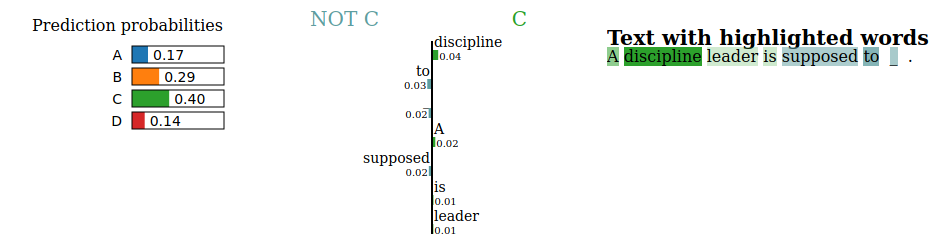
\includegraphics[scale=0.35]{images/lime-result-q-1a}
	\caption{\emph{LIME} result for the first experiment with original example.}
	\label{fig:lime-result-q-1a}
\end{figure}
\paragraph{}
In that example, the real label was $C$, and \emph{LIME} was able to detect that the important word was ``discipline'', so if we change this word the result will vary, but if we change the rest of the question, the result shouldn't change too much. 
So the next steps were to check if that idea was true. In order to do this some changes have been made in both the question and the options to see if the result is the same.
\paragraph{}

\section{Model-specific experiments}
\label{sec:ModelSpecificExperiments}
\noindent 
\subsection{Attention Heatmap}
\label{sec:AttentionHeatmapResults}
\noindent As said before, to visualize the \emph{Attention} values as a heatmap is a common method (first introduced in the original \emph{Attention} paper, \cite{Bahdanau2014}. 
\paragraph{}
To visualize the \emph{Attention} heatmap is an easy way to see how tokens relate with each others, which may help to understand what is going on inside the model. Although after several experiments (not only of this method but others, as wil be seen after) it has been seen that the \emph{Attention} values is not really useful to explain why the model has predict an specific output instead of another one, it can be used, as seen, to detect patterns, useless heads and so on.
\paragraph{}
As an explainability method it is true that it is not as helpful as other methods that are indeed trying to explain the model output. But it can be used to detect if the model is underfitted (or overfitted), which may explain a wrong prediction. But it does not help to explain a right prediction.
\paragraph{}
In this case a simple heatmap has been plotted to see how \emph{tokens} at the question attend to \emph{tokens} at each of the options. As the \emph{attention} heatmap takes the \emph{attention} values of each of the heads, it has been decided to make the sum of the values of each head to get a unique value of each \emph{token} relationship. This way, the heatmaps of figures \ref{fig:attention-heatmap-c} and \ref{fig:attention-heatmap-examples} shows the sum of the \emph{attention} values of each head of \emph{tokens} in x-axis attending to \emph{tokens} in y-axis.
\paragraph{}
As can be seen in Fig \ref{fig:attention-heatmap-c}, the \emph{discipline token} that is the most important one (according to other methods and having into account that is the \emph{token} that differs with other types of leaders in the text) has not a special value or relationships with other important \emph{tokens} in the sentence, such as \emph{nobody chats in class}. 
\begin{figure}[h]
	\centering
	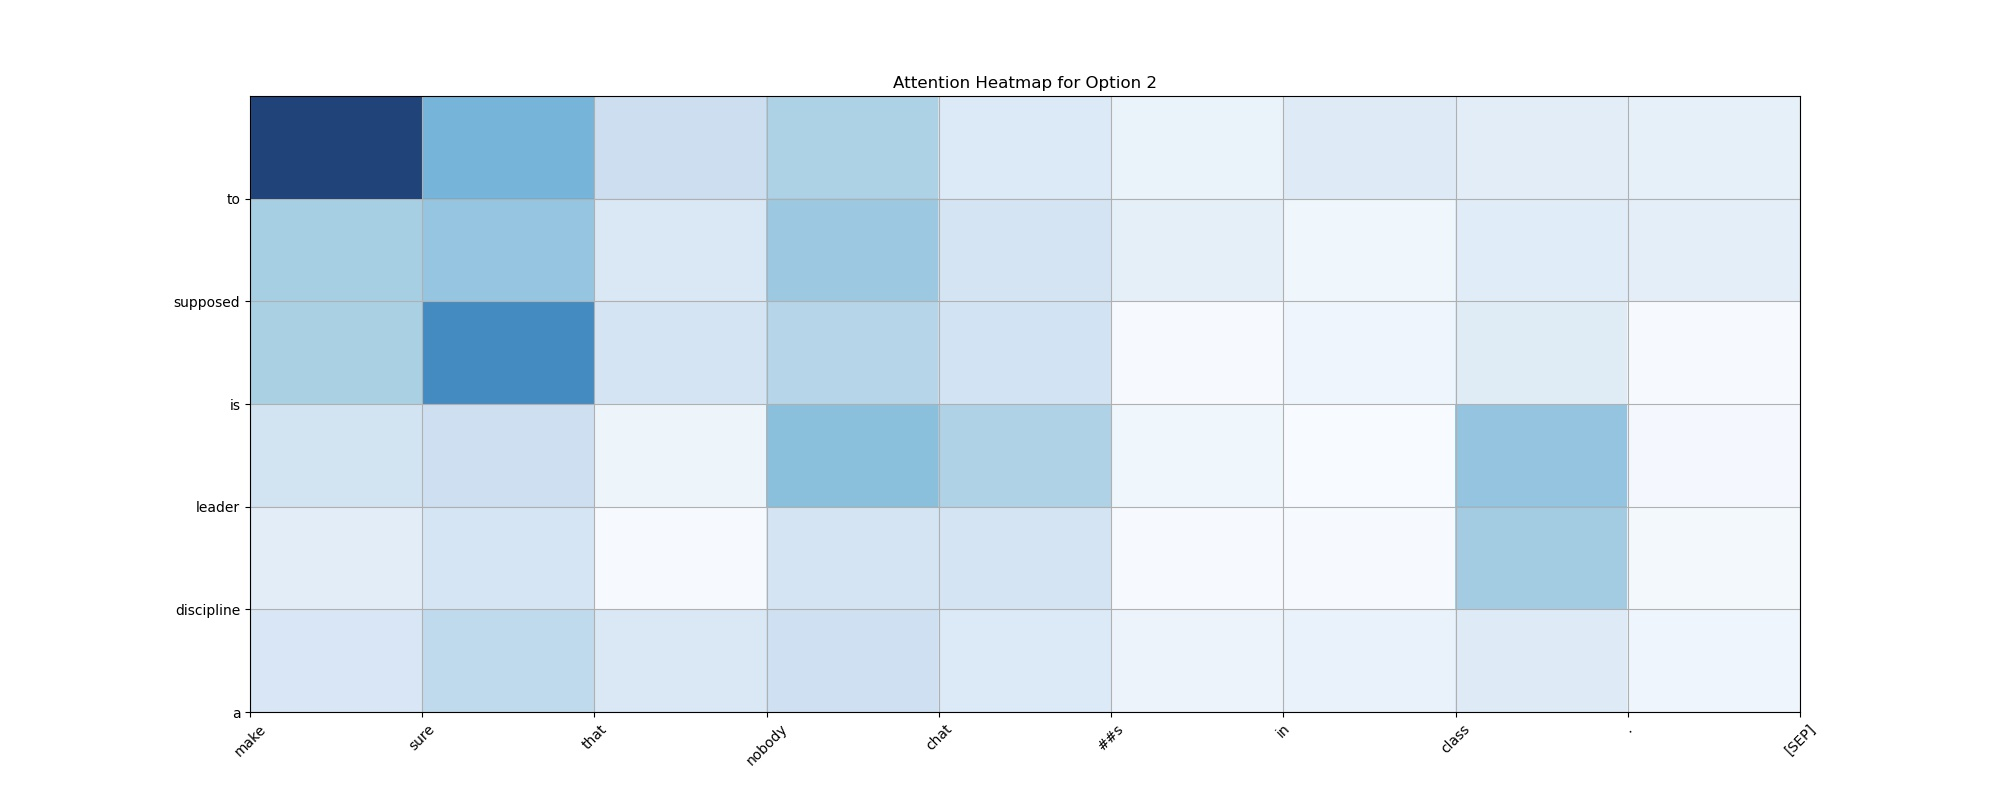
\includegraphics[scale=0.35]{images/attention_heatmap_2}
	\caption{\emph{Attention} heatmap for correct answer.}
	\label{fig:attention-heatmap-c}
\end{figure}
\paragraph{}
However, when looking at the heatmaps of other options, Fig \ref{fig:attention-heatmap-examples}, it can be seen that the \emph{discipline token} has higer values when attending to \emph{homework}, something that can have learnt during the training, as someone with discipline is someone that always does the homework. Also when looking at the whole picture (heatmap of each option), it can be seen that there is no a special pattern or something that helps to understand the model decision. 
\begin{figure}[h]
\centering
\begin{subfigure}{0.45\textwidth}
  \centering
	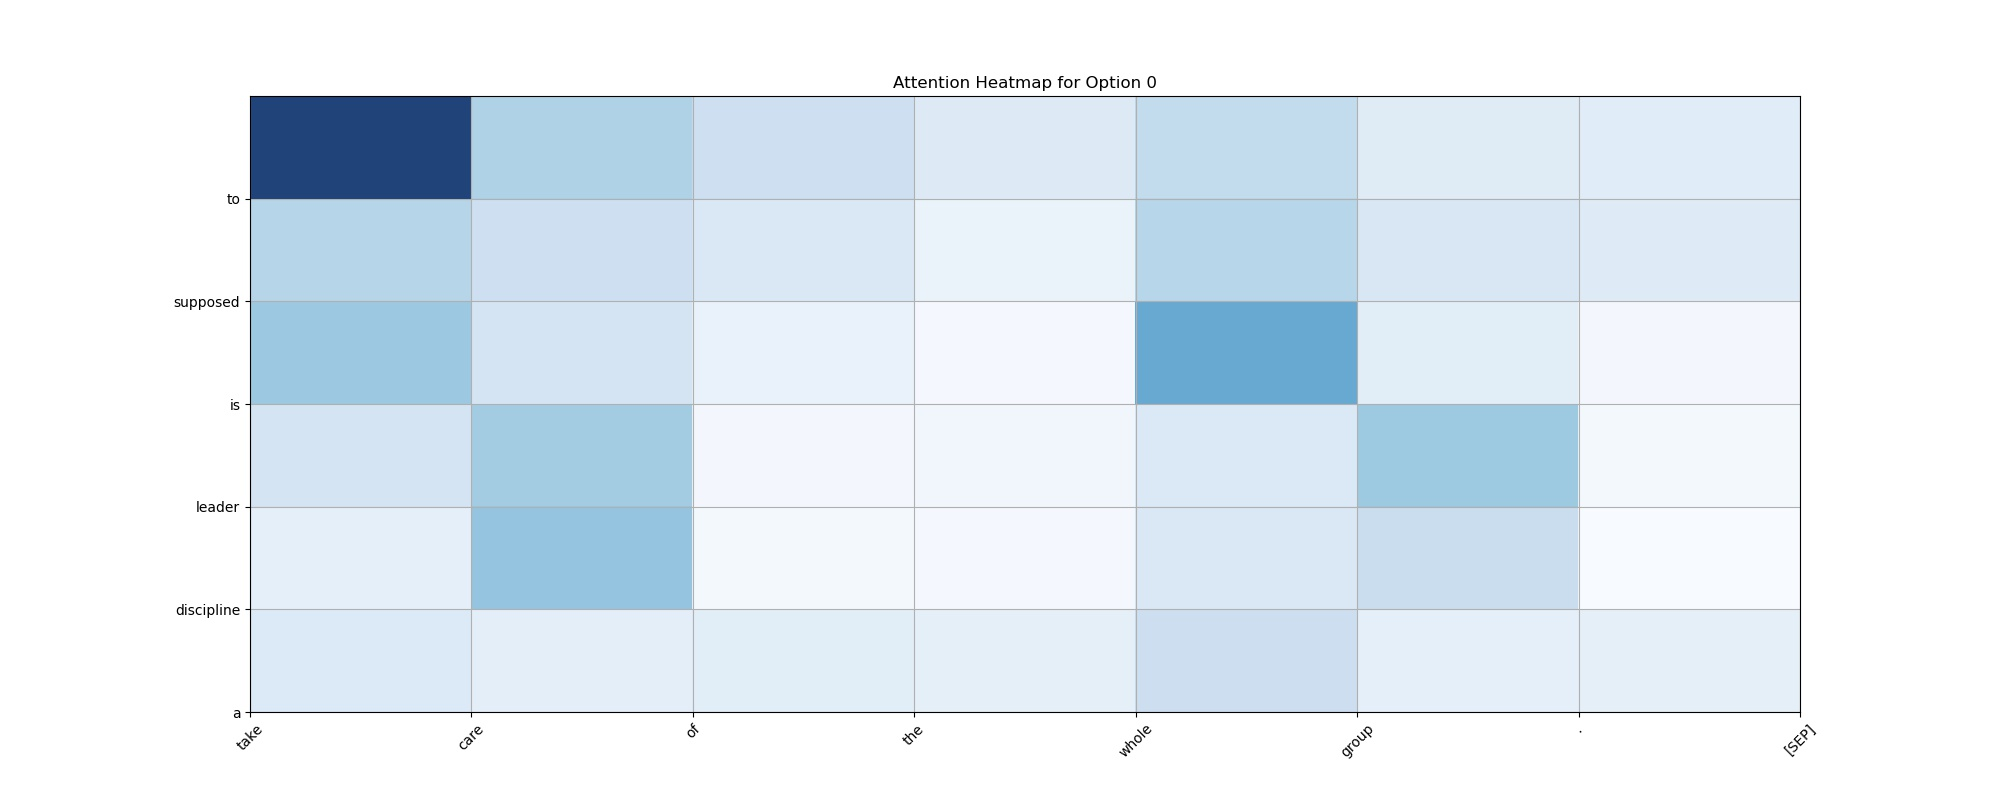
\includegraphics[width=200px]{images/attention_heatmap_0}
	\caption{\emph{Attention} heatmap option A.}
	\label{fig:att-hm-a}
\end{subfigure}
% \medskip\\
\begin{subfigure}{0.45\textwidth}
  \centering
	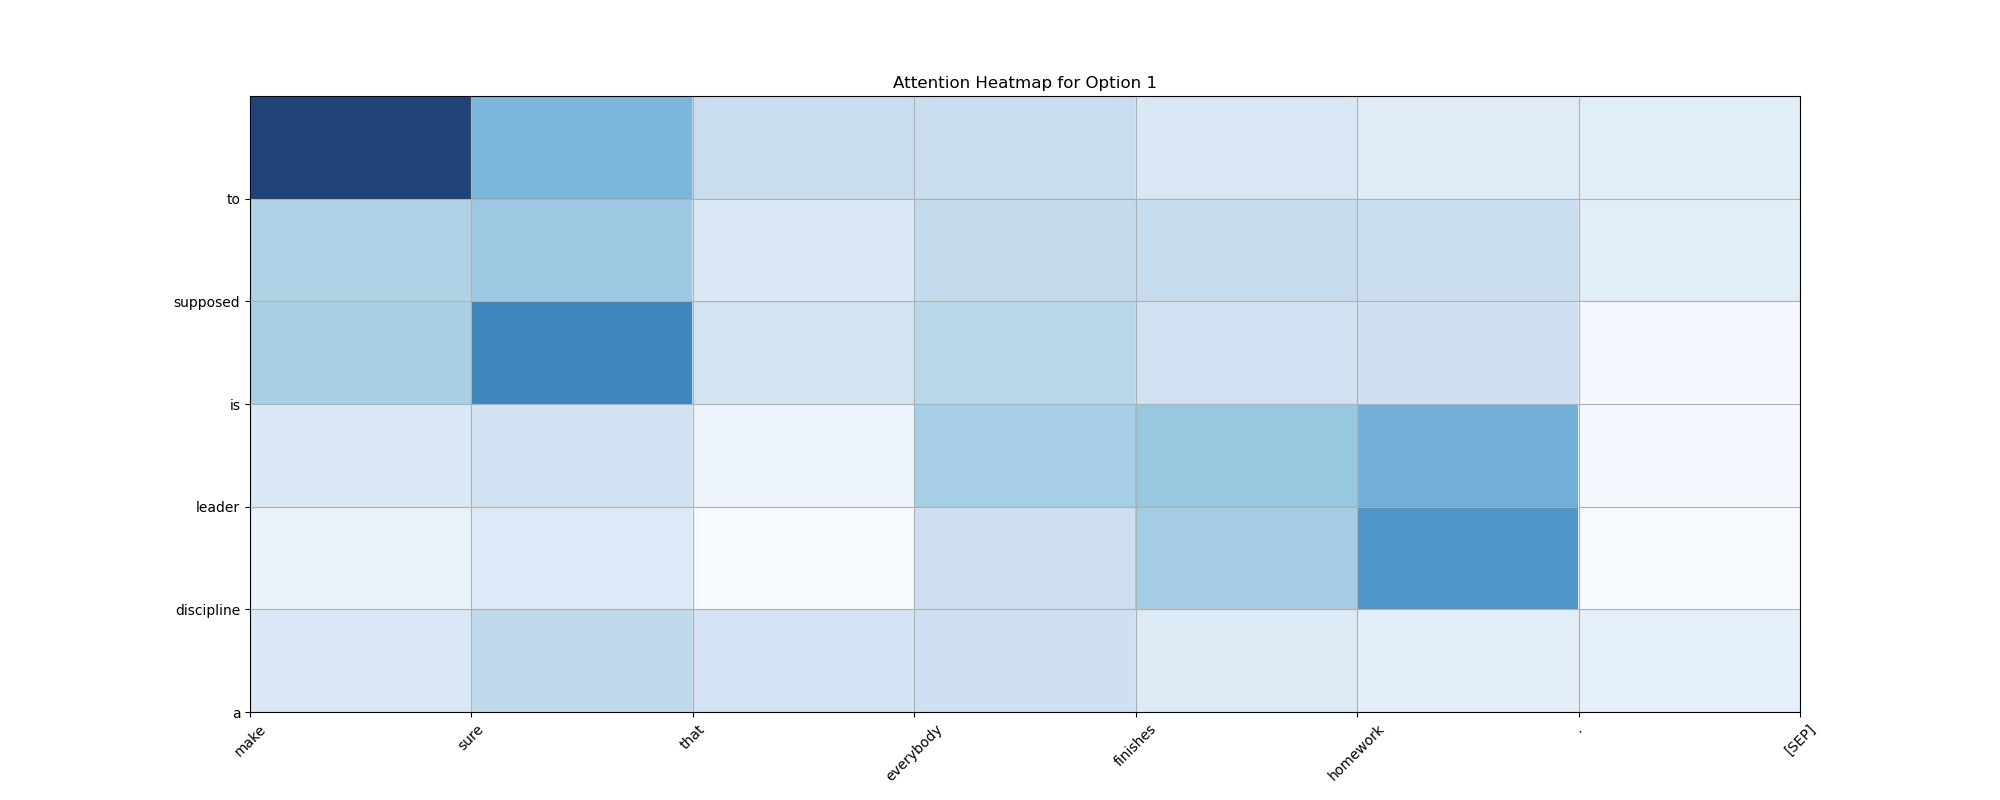
\includegraphics[width=200px]{images/attention_heatmap_1}
	\caption{\emph{Attention} heatmap option B.}
	\label{fig:att-hm-b}
\end{subfigure}
\medskip\\
\begin{subfigure}{0.45\textwidth}
  \centering
	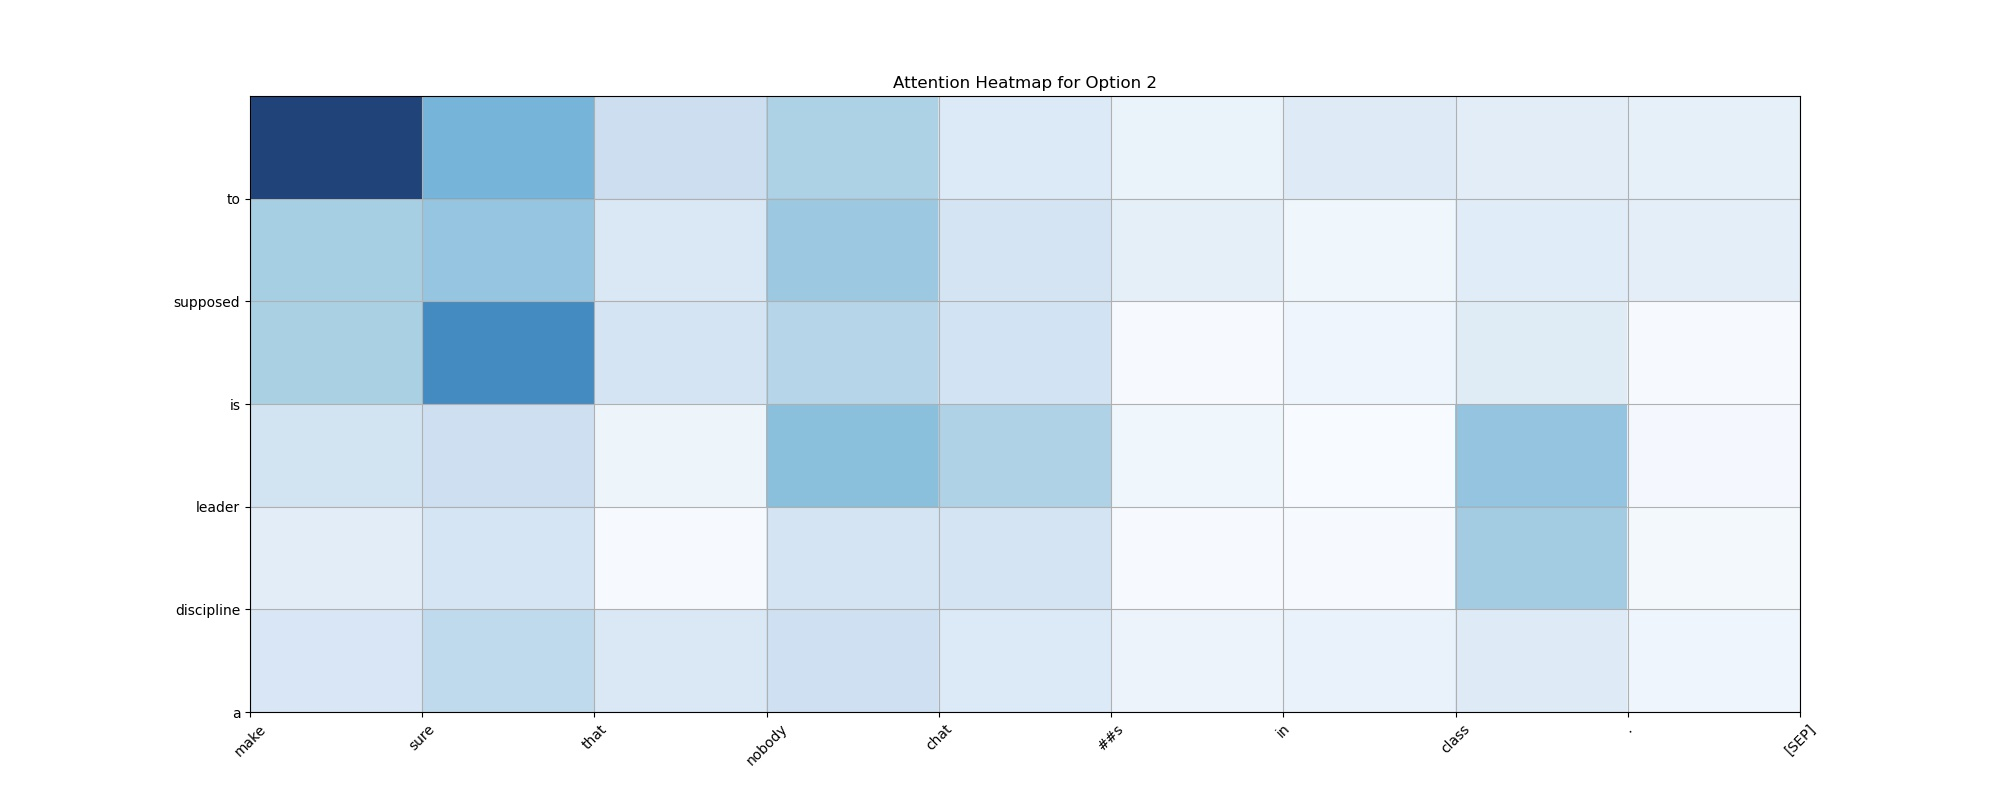
\includegraphics[width=200px]{images/attention_heatmap_2}
	\caption{\emph{Attention} heatmap option C.}
	\label{fig:att-hm-c}
\end{subfigure}
% \medskip\\
\begin{subfigure}{0.45\textwidth}
  \centering
	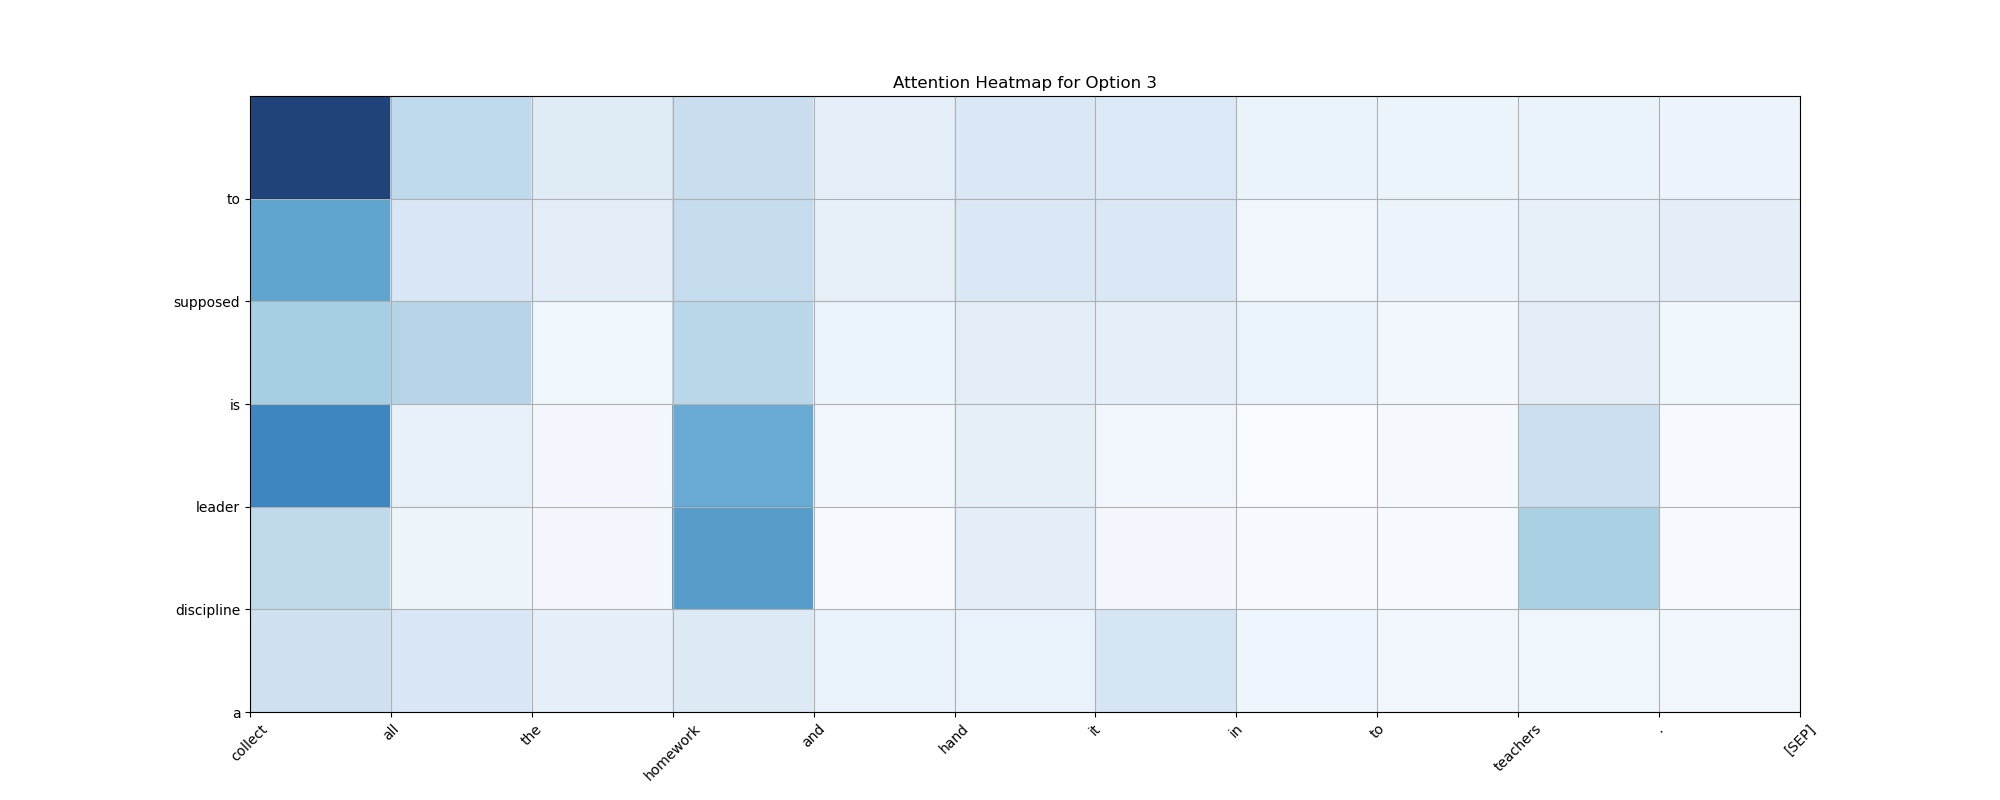
\includegraphics[width=200px]{images/attention_heatmap_3}
	\caption{\emph{Attention} heatmap option D.}
	\label{fig:att-hm-d}
\end{subfigure}
\caption{\emph{Attention} Heatmaps.}
\label{fig:attention-heatmap-examples}
\end{figure}


\subsection{BertViz}
\label{sec:BertVizResults}
\noindent Due to the problems of \emph{BertViz} to deal with large inputs, only has been tested the relations regarding the question and a single answer. This is, however, enough to test the tool, because it works in the same way no matter the input and, as it does not have to process anything, it does not matter the input used to test the tool and see how it works and how much information provides.
\paragraph{}
The first and most common way to study the \emph{Attention} layers is to use the \emph{Head View}, in which \emph{BertViz} shows the \emph{Attention} weights of a single layer. Again, the example used to test the tool has been: \textit{A discipline leader is supposed to  \_  .} 
\paragraph{}
When looking at how \emph{tokens} in Question attend to \emph{tokens} in each Answer, it can be seen that there is not anything that clarifies why the model chooses an option among the other. Figure \ref{fig:bertviz-q-options} shows layer 0 for each option. It can be seen that, for instance, \emph{discipline} attends more to \emph{tokens} such as \emph{class} or \emph{homework}, what makes sense. 
\begin{figure}[h]
\centering
\begin{subfigure}{0.4\textwidth}
  \centering
	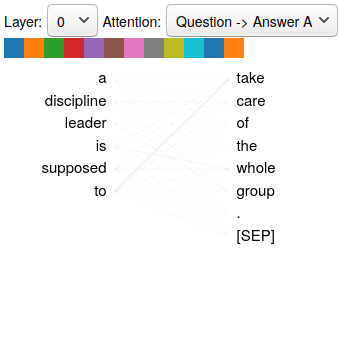
\includegraphics[width=120px]{images/bertviz-question-a}
	\caption{Question attending to Answer A.}
	\label{fig:bertviz-q-aa}
\end{subfigure}
\medskip
\begin{subfigure}{0.4\textwidth}
  \centering
	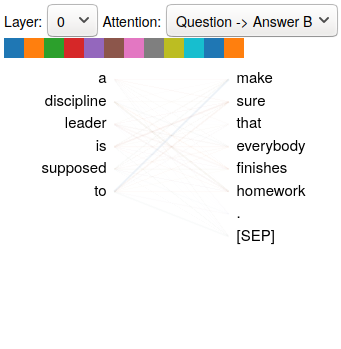
\includegraphics[width=120px]{images/bertviz-question-b}
	\caption{Question attending to Answer B.}
	\label{fig:bertviz-q-ab}
\end{subfigure}
\medskip\\
\begin{subfigure}{0.4\textwidth}
  \centering
	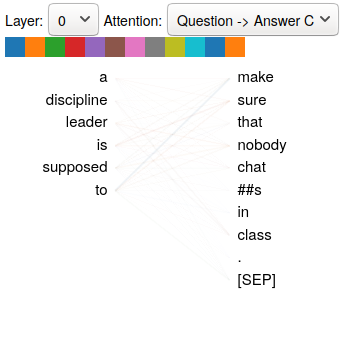
\includegraphics[width=120px]{images/bertviz-question-c}
	\caption{Question attending to Answer C.}
	\label{fig:bertviz-q-ac}
\end{subfigure}
\medskip
\begin{subfigure}{0.4\textwidth}
  \centering
	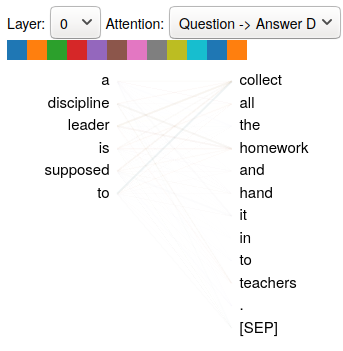
\includegraphics[width=120px]{images/bertviz-question-d}
	\caption{Question attending to Answer D.}
	\label{fig:bertviz-q-ad}
\end{subfigure}
\caption{\emph{BertViz} Head View of Question to Answers.}
\label{fig:bertviz-q-options}
\end{figure}
\paragraph{}
For instance, it can be seen in Figure \ref{fig:bertviz-l11h2} that \emph{discipline} attends to \emph{make sure that nobody}, which is really related to \emph{discipline}. However, there are different patterns across the layers and heads, and each head in each layer attend to \emph{tokens} by following a specific pattern. 
\begin{figure}[!h]
	\centering
	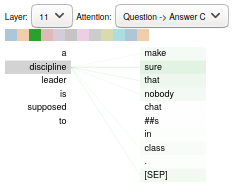
\includegraphics[scale=0.4]{images/bertviz-question-l11-head2}
	\caption{\emph{BertViz} layer 11, head 2.}
	\label{fig:bertviz-l11h2}
\end{figure}
\paragraph{}
As there are usually too many heads (model used has 12 heads per each one of the 12 layers), it costs a lot to look at each one separately. In order to take a global look and to discover patterns and useless heads, the \emph{BertViz Model View} is used. In Figure \ref{fig:bertviz-model-q} it can be seen that the \emph{Attention} layers follow patterns, even when the option change.
\begin{figure}[!h]
\centering
\begin{subfigure}{0.4\textwidth}
  \centering
	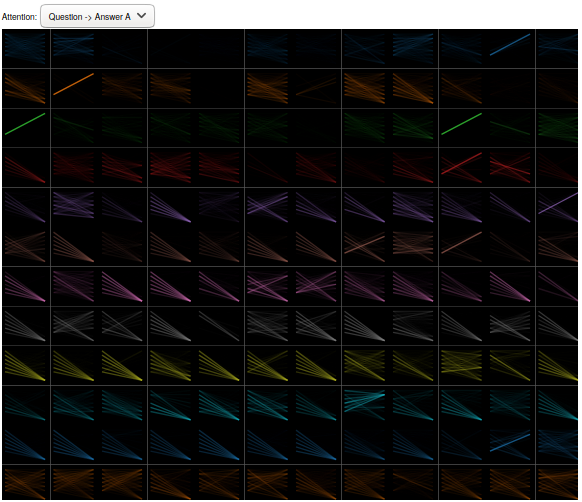
\includegraphics[width=140px]{images/bertviz-model-a}
	\caption{Question attending to Answer A.}
	\label{fig:bertviz-model-q-aa}
\end{subfigure}
\medskip 
\begin{subfigure}{0.4\textwidth}
  \centering
	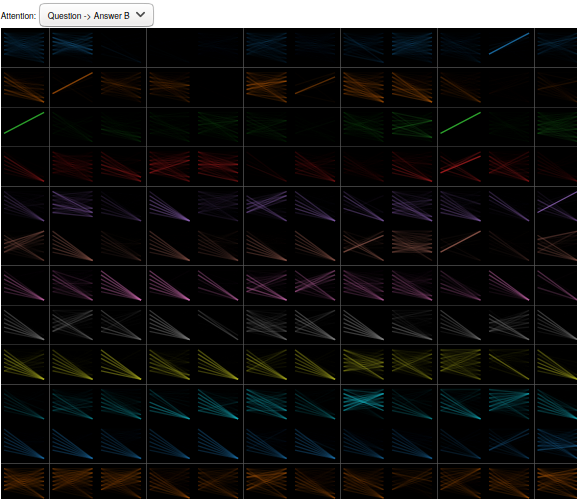
\includegraphics[width=140px]{images/bertviz-model-b}
	\caption{Question attending to Answer B.}
	\label{fig:bertviz-model-q-ab}
\end{subfigure}
\caption{\emph{BertViz} Model View of Question to Answers A and B.}
\label{fig:bertviz-model-q}
\end{figure}
\paragraph{}
Once that a pattern have been detected (or an outlier) it's useful to look at that specific head. The tool let the user to do this by clicking in the corresponding head, Figure \ref{fig:bertviz-model-head}. This way the user can see what \emph{tokens} are being attended at in the patterns, e.g. nouns, prepositions, etc. 
\begin{figure}[!h]
	\centering
	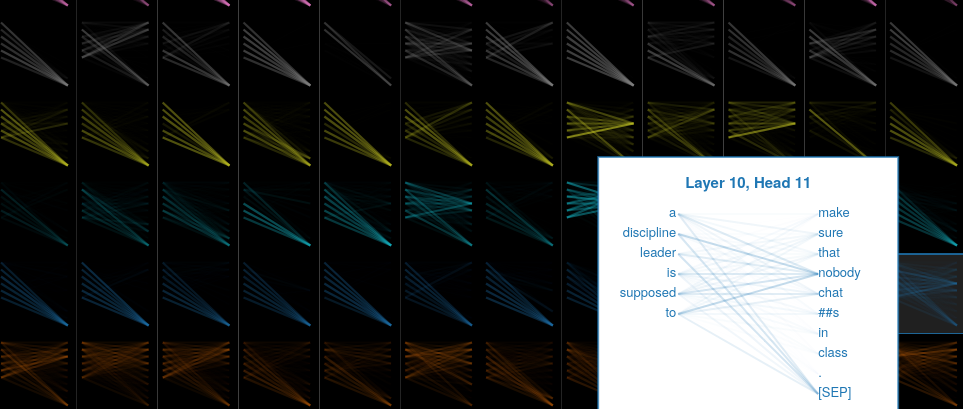
\includegraphics[scale=0.4]{images/bertviz-model-detail}
	\caption{To look at a single head in the Model View of \emph{BertViz}.}
	\label{fig:bertviz-model-head}
\end{figure}
\paragraph{}
The model view is useful to have a global look of the model, to see its behaviour and to see what heads are useful/useless. For instance, it can be seen that a lot of heads follow the same pattern, all \emph{tokens} attend to the \emph{[SEP] token}, what is considered as a \emph{null head}. These heads, therefore, could be prune to save space and time. This could be due to the training of the model, meaning that the model could be underfitted and, therefore, should be trained with more data or during more time, which in this case is true, because due to hardware and temporal limitations the model has been training for just 1 day, which is not enough for a \emph{LM}.
\paragraph{}
Therefore, to look at the \emph{Attention} does not really provide an explanation of why the model choose one option, because it follows patterns and does not change over the different options. 
\paragraph{}
Although \emph{BertViz} does not help to explain a prediction of the model, it is a good tool for visualizing the \emph{Attention} weights, what can be useful as said before to, for instance, prune useless heads. But it's not a good option for explain a prediction of the model.

\cleardoublepage
\subsection{Intrinsic GPT-3}
\label{sec:GPT3Results}
\noindent To force \emph{GPT-3} to generate the explanations (or any expected result), first a few examples of what exactly is desired have to be feed to the model in order to show it what is expected.
\paragraph{}
In this case, three passages were selected from the test set to feed \emph{GPT-3} and force it to generate the text as wished, this is, an explanation of the answer. These passages were complex to answer, beacuse in some of them the answer was not in the text itself, but related to. For instance, in one of the passages the question asks about the location of the story, given as options: England; America; Japan; Australia. But in the text it talks about New York, so a bit of commonsense is needed in order to relate New York with America.
\paragraph{}
The examples feed to the model included the context, the question, the options, the correct answer and a simple explanation of why it is the correct answer. The appendix \ref{ch:GPT3-Examples} includes all the examples feed to the model. 
\paragraph{Example 1}
The first try was using the Example 1, \ref{ex:1}. As the answer was in the text it was not surprising that \emph{GPT-3} predicted it correctly. Regarding the explanation, Figure \ref{fig:gpt3-ex1}, it is a good explanation but, again, as the answer is inside the text there was not too much to explain but say that the article says so.
\begin{figure}[h]
	\centering
	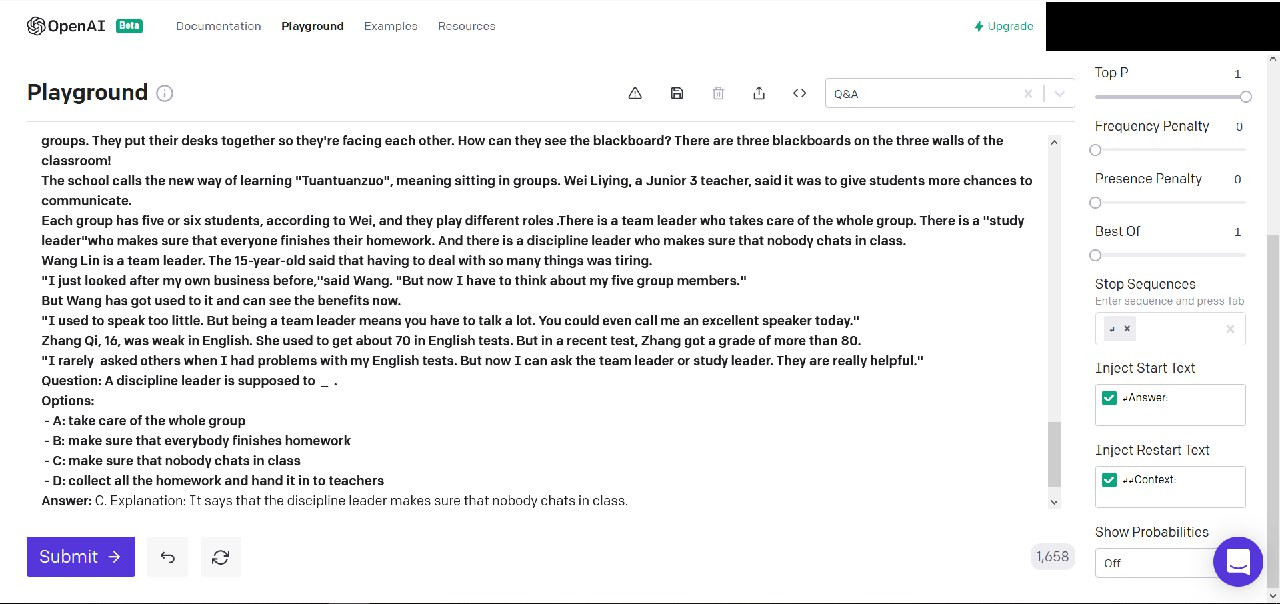
\includegraphics[scale=0.25]{images/gpt3-ex1}
	\caption{Explanation of GPT3 for the Example 1.}
	\label{fig:gpt3-ex1}
\end{figure}
\paragraph{Example 2}

\paragraph{}
Surprisngly, the result of \emph{GPT-3} included the correct answer and an accurately explanation, \ref{fig:gpt3-result-correct}.
\begin{figure}[h]
	\centering
	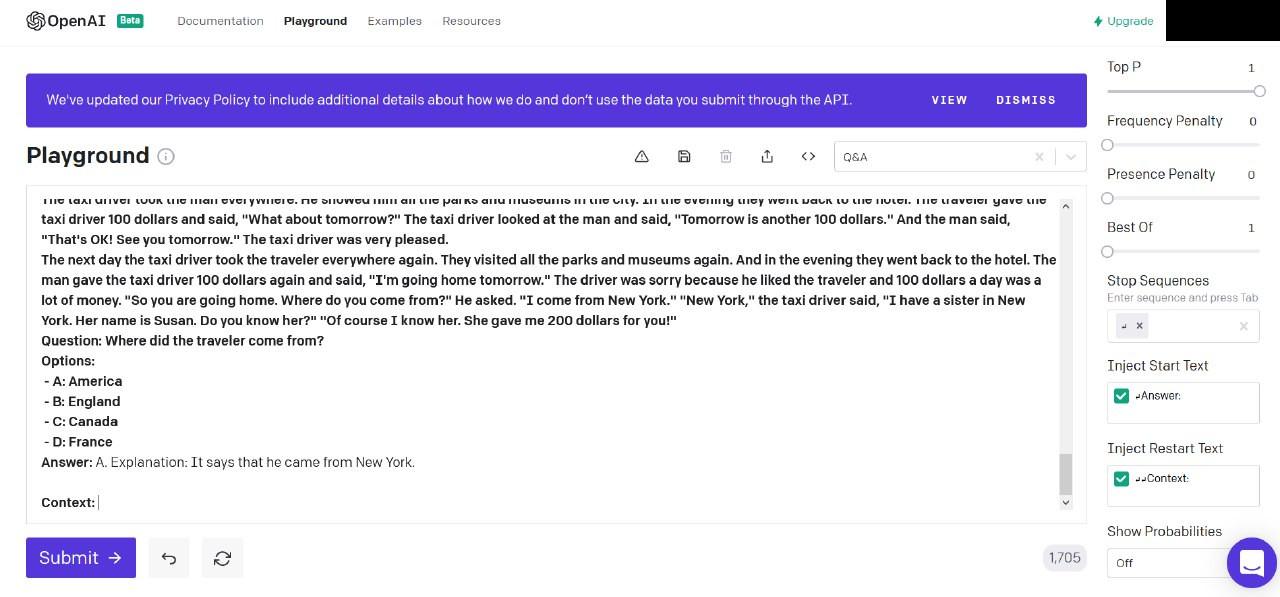
\includegraphics[scale=0.25]{images/gpt3-correct}
	\caption{Explanation of GPT3.}
	\label{fig:gpt3-result-correct}
\end{figure}
\paragraph{}
But it has been detected that it is not always that good, and therefore it is not clear if it's indeed able to explain itself. With a simple change of options, interchanging the options A and B, the result fails in the prediction, the explanation is the same though, \ref{fig:gpt3-result-fail1}. And if an extra ``answer'' token is added to the end, the result of the prediction is correct but it fails in the explanation, \ref{fig:gpt3-result-fail2}.
\begin{figure}[h]
	\centering
	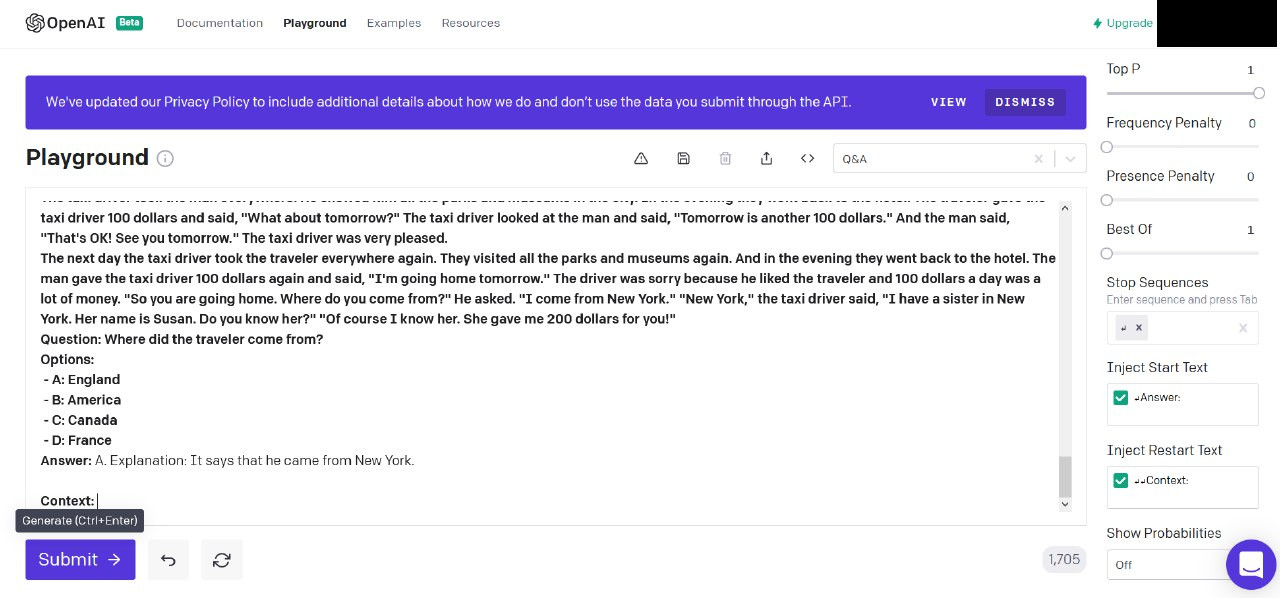
\includegraphics[scale=0.25]{images/gpt3-fail1}
	\caption{Wrong prediction of GPT3.}
	\label{fig:gpt3-result-fail1}
\end{figure}
\begin{figure}[h]
	\centering
	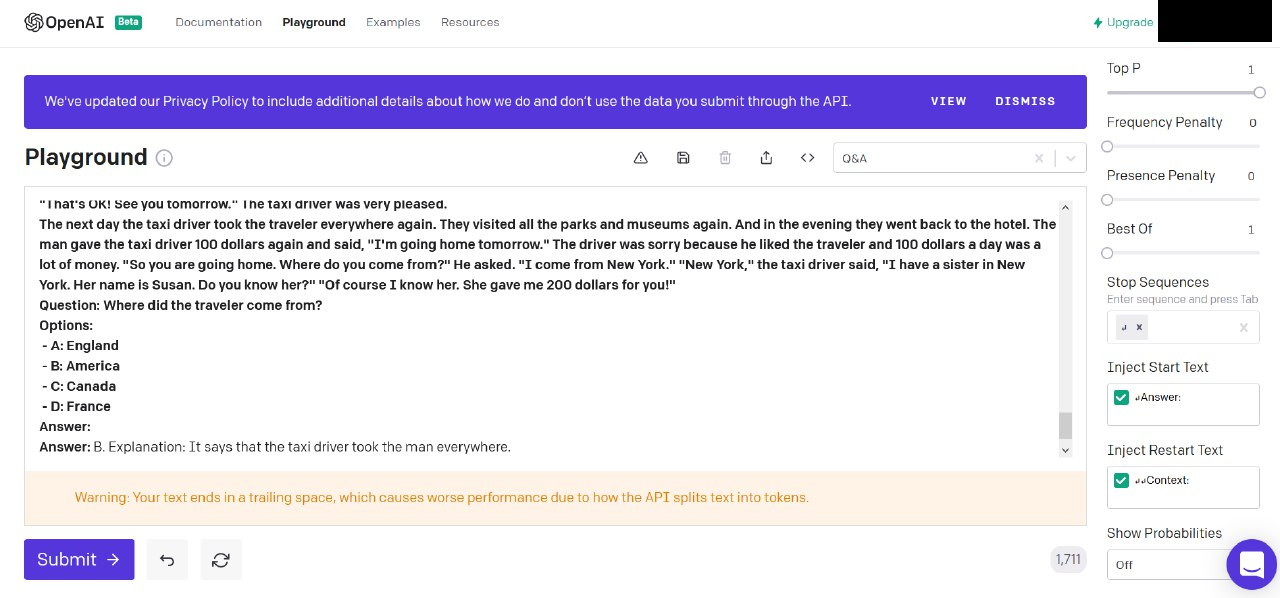
\includegraphics[scale=0.25]{images/gpt3-fail2}
	\caption{Wrong explanation of GPT3.}
	\label{fig:gpt3-result-fail2}
\end{figure}